\chapter{Stream Editor}
\labch{sed}

\begin{marginfigure}
  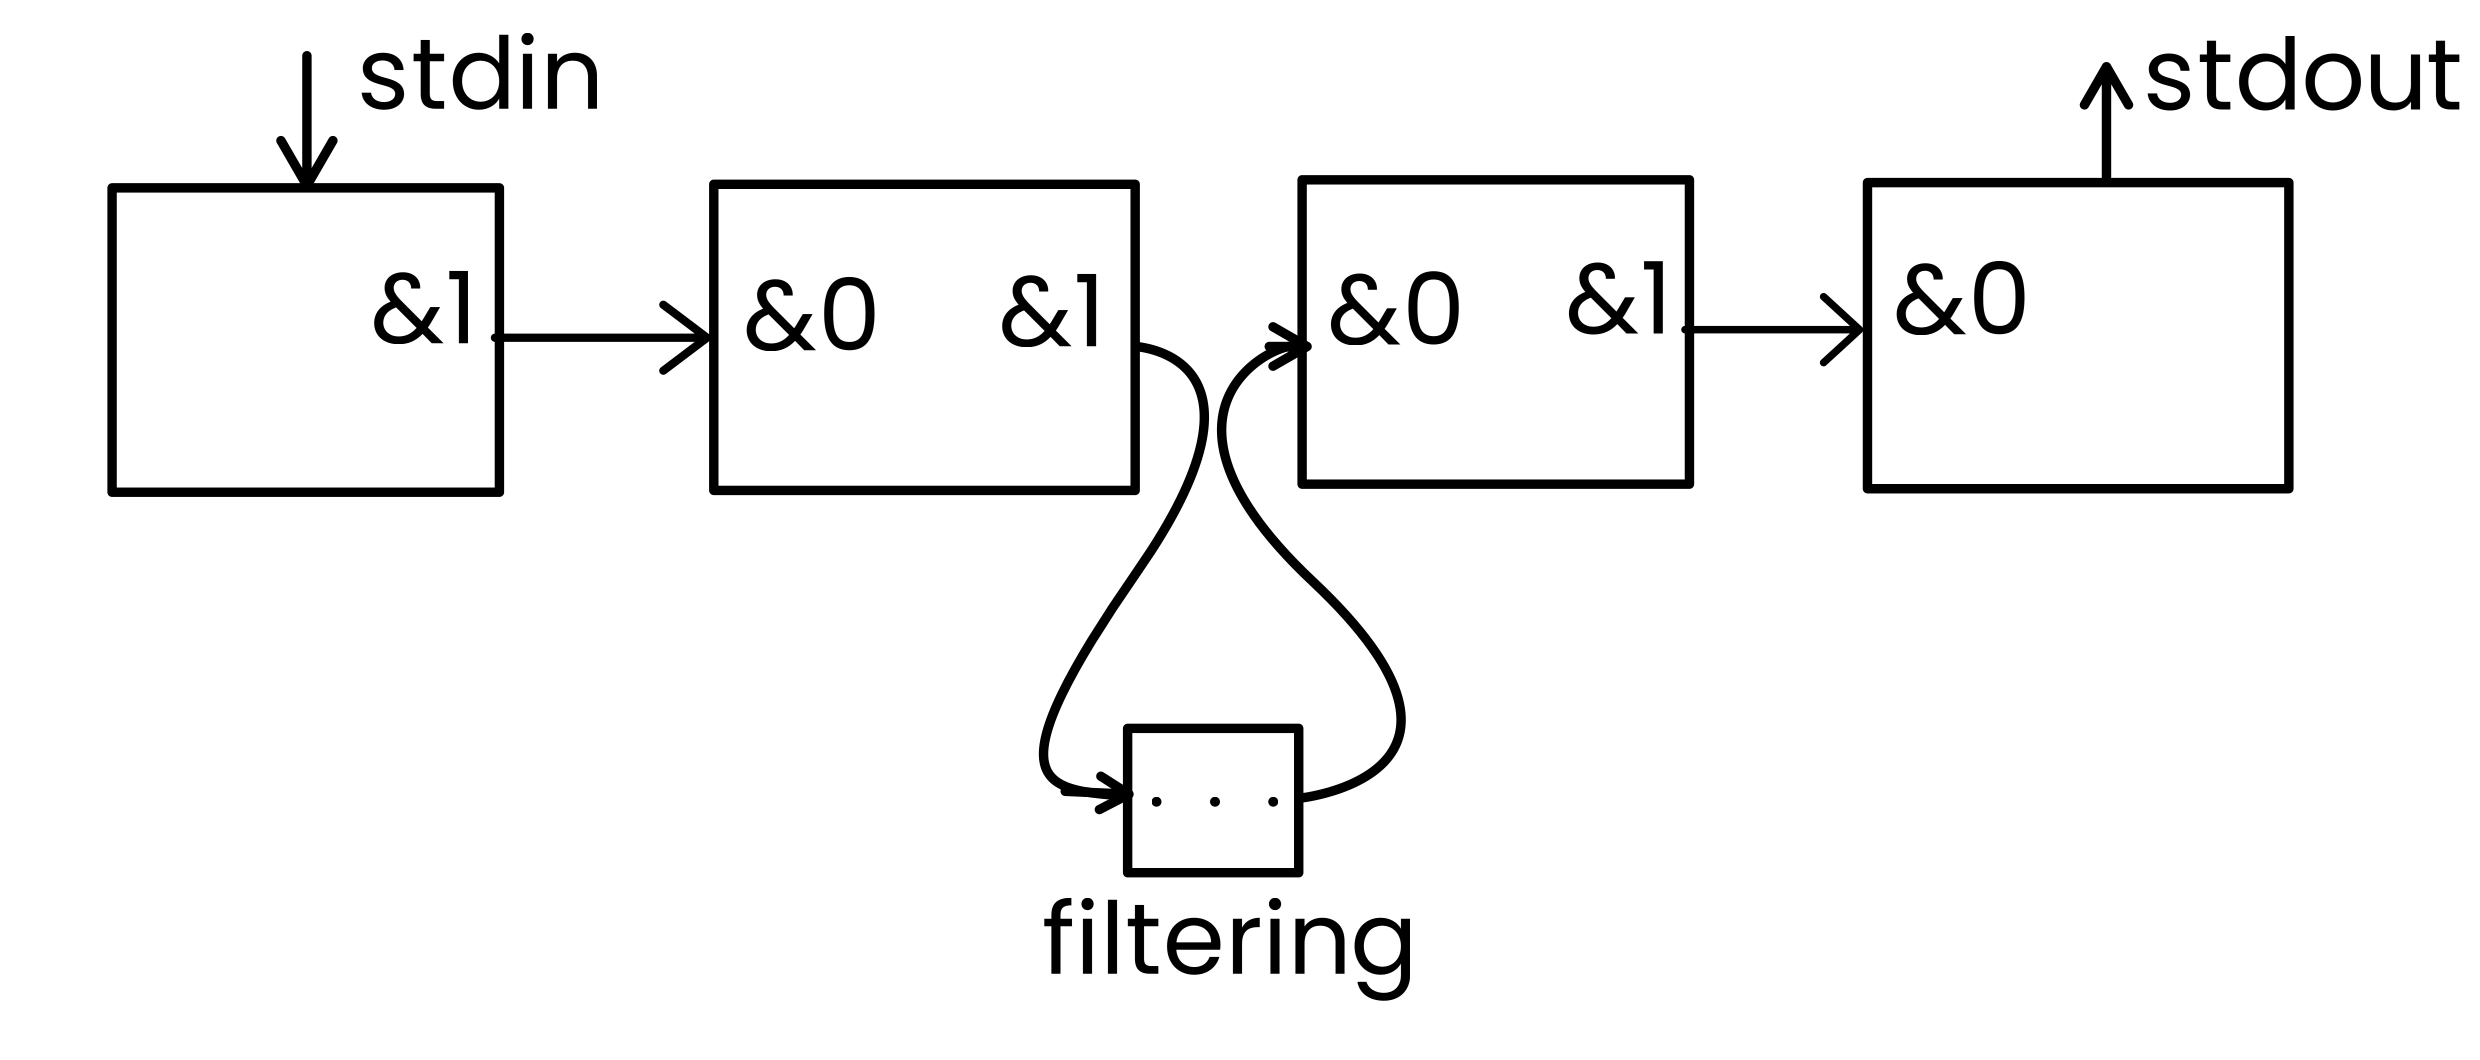
\includegraphics{filtering}
  \caption{Filtering Streams}
  \labfig{filtering}
\end{marginfigure}

\textbf{Stream Editor} (sed) is a powerful text stream editor. It is used to perform basic text transformations on an input stream (a file or input from a pipeline). While in some ways similar to an editor which permits scripted edits (such as ed), sed works by making only one pass over the input(s), and is consequently more efficient. But it is sed's ability to filter text in a pipeline which particularly distinguishes it from other types of editors.

This means that sed can be used in a pipeline of other commands to filter, refine, and transform the data in the stream. This is illustrated in \reffig{filtering}.

\begin{remark}
\lstinline|sed| is short for \textbf{S}tream \textbf{ED}itor.
\end{remark}

\section{Basic Usage}

\begin{marginfigure}[-3cm]
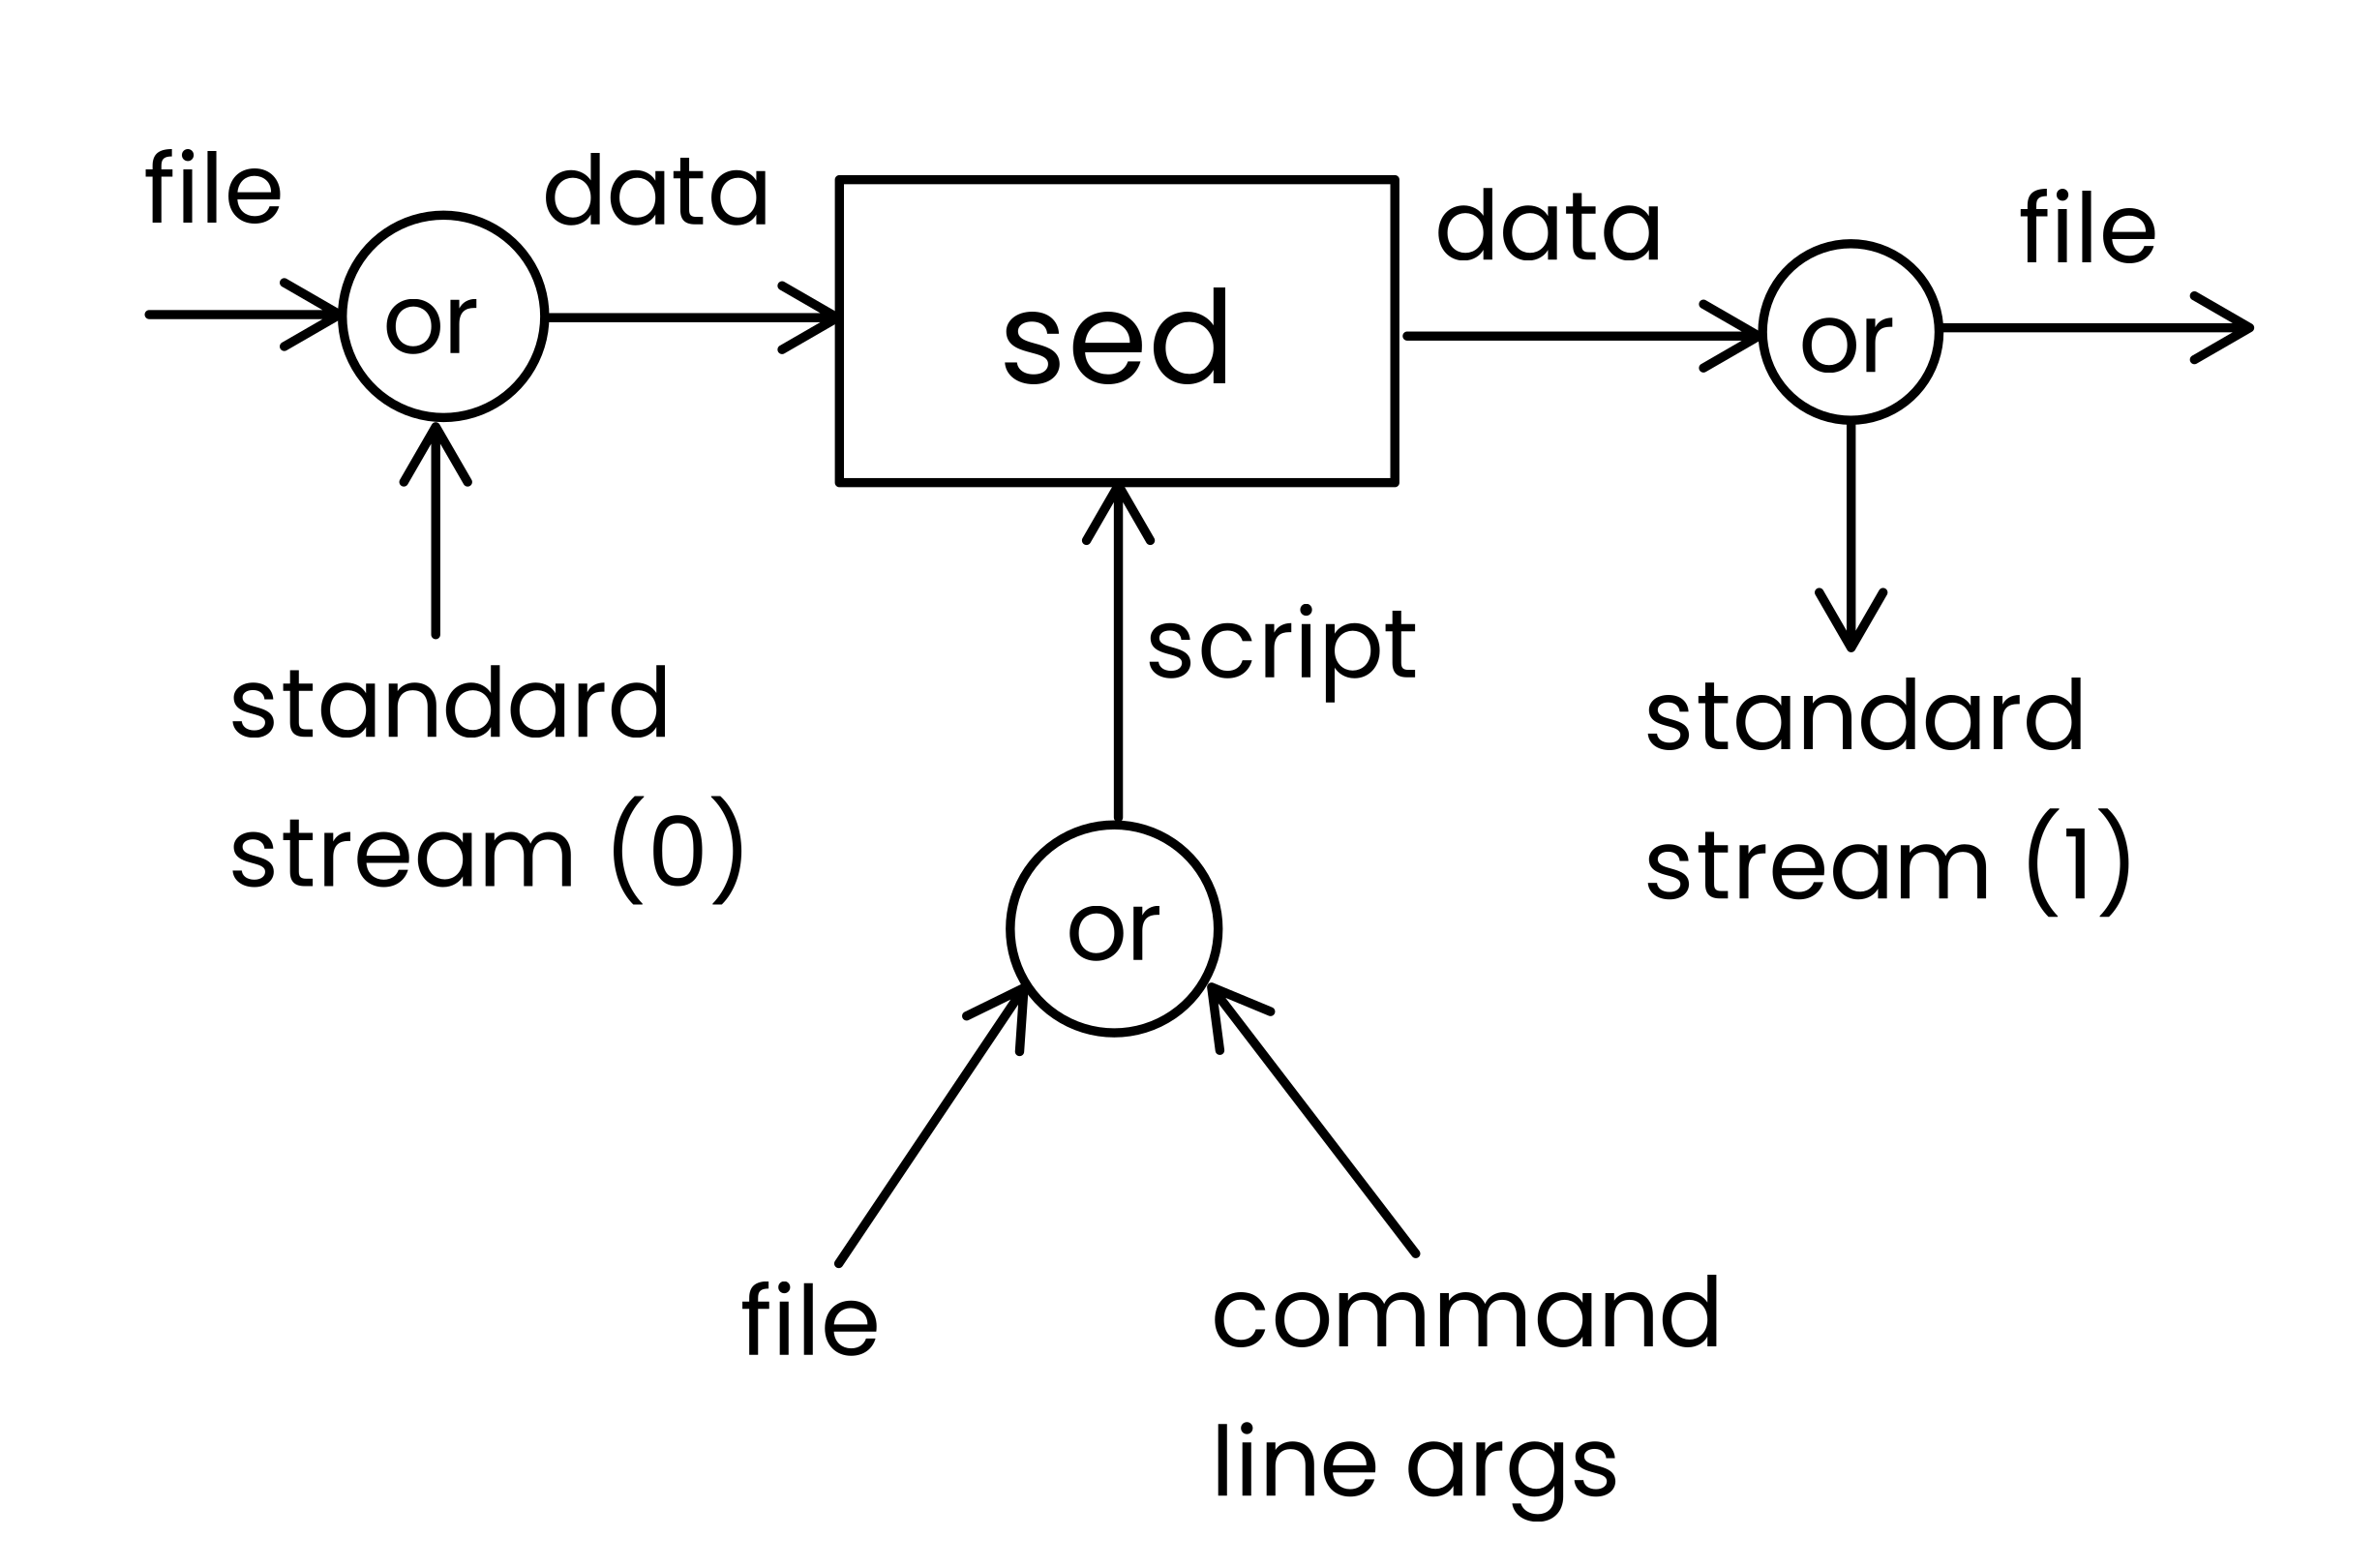
\includegraphics{sed}
\caption{The different interfaces to sed}
\labfig{sed}
\end{marginfigure}

Sed needs an input (stream or file) and a script to work. The script is a series of commands that sed will execute on the input. The script can be passed as a command line argument or as a file as well.

For example, we can provide the stream to manipulate as standard input, and provide a single command as the script directly through the command line.

\marginnote{
  Here we are using the \lstinline|s| command of sed to perform a find-and-replace style substitution. This is similar to the \lstinline|\%s/regex/string/| present in \lstinline|vim|.
  The first argument can be a regex, but the second argument has to be a string, however it may contain backreferences to the matched pattern.
}
\begin{lstlisting}[language=bash]
$ sed 's/World/Universe/' <<< "Hello World"
Hello Universe
\end{lstlisting}

As sed can work on standard input if no file is provided, it is very useful when paired with other tools; It can transform or filter output of commands.

For example, the default output of date does not zero-pad the date.
If we want to do that using \lstinline|sed|, we can do it as follows:

\marginnote{
  This does not add an extra zero if the date is already two digits long.
  As we have already covered regular expressions in depth, it should be easy to understand the regex used here. We are grouping the regex to use it in the back reference and add an extra zero if the date is a single digit.
}
\begin{lstlisting}[language=bash]
$ date
Tue Aug  6 05:00:23 PM IST 2024
$ date | sed -E 's/^([[:alpha:]]*[[:space:]]*[[:alpha:]]*)[[:space:]]*([[:digit:]])[[:space:]]/\1 0\2 /'
Tue Aug 06 05:00:32 PM IST 2024
$ date -d "20241225"
Wed Dec 25 12:00:00 AM IST 2024
$ date -d "20241225" | sed -E 's/^([[:alpha:]]*[[:space:]]*[[:alpha:]]*)[[:space:]]*([[:digit:]])[[:space:]]/\1 0\2 /'
Wed Dec 25 12:00:00 AM IST 2024
\end{lstlisting}

If the pattern being searched does not match on the input, sed will not make any changes to the input.

\section{Addressing}

All of the commands in \lstinline|sed| runs on all the lines by default.
However, we can specify the lines to run on by providing the optional address field before the command.

\begin{lstlisting}[language=bash]
$ cat data
hello world
hello universe
$ sed '1s/hello/hi/' data
hi world
hello universe
\end{lstlisting}

The address can be the line number of a particular line, range of line numbers, or a regex pattern to match. We can also use \lstinline|$| to match the last line and \lstinline|1| to match the first line.

\begin{lstlisting}[language=bash]
$ seq 10 20 | sed '5,10d'
10
11
12
13
20
\end{lstlisting}

\begin{lstlisting}[language=bash]
$ seq 10 20 | sed '/15/,/20/d'
10
11
12
13
14
\end{lstlisting}

\begin{lstlisting}[language=bash]
$ seq 10 20 | sed '5d'
10
11
12
13
15
16
17
18
19
20
\end{lstlisting}


Furthermore, we can also specify the range of addresses to run the command on, using regex as the start, end, or both the ends.

\begin{lstlisting}[language=bash]
$ seq 10 20 | sed '/13/,$d'
10
11
12
\end{lstlisting}

The range usually uses the start and end addresses separated by a comma. But we can also use \lstinline|+n| to include \lstinline|n| lines starting from the start range.

\begin{lstlisting}[language=bash]
$ seq 10 20 | sed '/13/,+5d'
10
11
12
19
20
\end{lstlisting}

To match every \lstinline|n|th line, we can use \lstinline|~n|.

\begin{lstlisting}[language=bash]
$ seq 10 20 | sed '0~2d'
10
12
14
16
18
20
\end{lstlisting}

\subsection{Negation}

We can negate the address by using the \lstinline|!| operator before the address.

\begin{lstlisting}[language=bash]
$ seq 8 5 32 | sed '/1./!d'
13
18
\end{lstlisting}

In this example we first use the \lstinline|seq| command to generate a sequence of numbers from 8 to 32 with a step of 5.
Then we use \lstinline|sed| to delete all the lines that do not match the pattern \lstinline|1.|, printing only the numbers that start with $1$.

\section{Commands}

\subsection{Command Syntax}

The general syntax of the sed command is as follows:

\begin{lstlisting}[language=bash]
[:label] [address] command [arguments]
\end{lstlisting}

\subsection{Available Commands}

Sed has a lot of commands that can be used to manipulate the input stream. Here are some of the most commonly used commands:

\begin{itemize}
  \item \lstinline|p| - Print the pattern space.
  \item \lstinline|d| - Delete the pattern space.
  \item \lstinline|s| - Substitute the pattern using regex match with string. \\
    \lstinline|[address]s/search regex/replace string/[flags]|
  \item \lstinline|=| - Print the current line number.
  \item \lstinline|#| - Comment.
  \item \lstinline|i| - Insert text before the current line.
  \item \lstinline|a| - Insert text after the current line.
  \item \lstinline|c| - Change the current line.
  \item \lstinline|y| - Transliterate the characters in the pattern space.
  \item \lstinline|q [exit code]| - Quit the script.
\end{itemize}

\subsection{Branching and Flow Control}
Other than these, there are other control flow commands like \lstinline|b|, \lstinline|t|, \lstinline|:|, which let us create more complex and powerful transformations with state information.

\begin{itemize}
  \item \lstinline|b label| - Branch unconditionally to label.
  \item \lstinline|:label| - Define Label for branching.
  \item \lstinline|n| - Read the next line to the pattern space.
  \item \lstinline|N| - Append the next line to the pattern space.
  \item \lstinline|t label| - Branch to label on successful substitution.
  \item \lstinline|T label| - Branch to label on failed substitution.
  \item \lstinline|w file| - Write the pattern space to file.
  \item \lstinline|r file| - Append the contents of file to the pattern space.
  \item \lstinline|h| - Copy the pattern space to the hold space.
  \item \lstinline|H| - Append the pattern space to the hold space.
  \item \lstinline|g| - Copy the hold space to the pattern space.
  \item \lstinline|G| - Append the hold space to the pattern space.
  \item \lstinline|x| - Exchange the pattern space and the hold space.
  \item \lstinline|D| - Delete the first line of the pattern space.
  \item \lstinline|P| - Print the first line of the pattern space.
\end{itemize}

More details on these commands can be found in the \lstinline|man| and \lstinline|info| pages of \lstinline|sed|.

\subsection{Printing}

The \lstinline|p| command prints a line in sed.
By default the line in pattern space is printed by default.
However this can be suppresesed using the \lstinline|-n| flag.
Thus when the \lstinline|p| command is used along with the \lstinline|-n| flag, only the lines that are explicitly printed are shown.

\begin{lstlisting}[language=bash]
$ seq 10 20 | sed -n '5p'
14
\end{lstlisting}

\subsection{Deleting}

The \lstinline|d| command deletes the line in the pattern space.
This is useful if the \lstinline|-n| flag is not used to suppress the default printing.

\marginnote{
  Here we are deleting two ranges of lines from the input stream.
  Multiple commands can be separated by a semicolon.
}
\begin{lstlisting}[language=bash]
$ seq 10 20 | sed '1,4d;6,$d'
14
\end{lstlisting}

Thus there are two ways of filtering a stream of data as seen in the last two examples:
\begin{itemize}
  \item Print only the lines that match a pattern.
  \item Delete the lines that do not match a pattern.
\end{itemize}

\begin{remark}
  If we use the \lstinline|p| command without using the \lstinline|-n| flag, the matched lines will be printed twice, and the other lines will be printed once.
\end{remark}

\begin{lstlisting}[language=bash]
$ seq 1 5 | sed '2p'
1
2
2
3
4
5
\end{lstlisting}

\subsection{Substitution}

This is one of the most widely used commands in \lstinline|sed|.
The sustitute command is used to replace a pattern with a string.
The search pattern can be a fixed string, or a regex pattern.

\begin{remark}
  \lstinline|sed| supports two types of regex: Basic and Extended.
  Perl Compatible Regular Expressions (PCRE) are not supported by \lstinline|sed|.
\end{remark}

Like the other commands, the substitution command can be used with an address to specify the lines to run on, or on all the lines.

\begin{lstlisting}[language=bash]
$ seq 8 12 | sed 's/1/one/'
8
9
one0
one1
one2
\end{lstlisting}

Observe that although the pattern \lstinline|1| is present twice in 11, it is only replaced once as the substitution command only replaces the first occurrence of the pattern in the line.

To substitute all the occurrences of the pattern in the line, we can use the \lstinline|g| option to the \lstinline|s| command.

\begin{lstlisting}[language=bash]
$ seq 8 12 | sed 's/1/one/g'
8
9
one0
oneone
one2
\end{lstlisting}

The \lstinline|g| argument stands for global, and it replaces all the occurrences of the pattern in the line.

If we want to replace only the \lstinline|n|th occurrence of the pattern, we can mention the number instead of \lstinline|g|.

\begin{lstlisting}[language=bash]
$ seq 8 12 | sed 's/1/one/2'
8
9
10
1one
12
\end{lstlisting}

Here the \lstinline|2| flag replaces the second occurrence of the pattern in the line.

Observe that the lines with only one occurrence of the pattern are not changed at all.

\begin{remark}
 If we ask \lstinline|sed| to replace the \lstinline|n|th occurrence of the pattern, and the pattern does not occur the pattern \lstinline|n| times in the line, then the line is not changed at all.
\end{remark}

\subsubsection{Case Insensitive Substitution}

If we want to perform a case insensitive substitution, we can use the \lstinline|i| option to the \lstinline|s| flag.

\begin{lstlisting}[language=bash]
$ sed 's/Hello/Hi/i' <<< "hello world"
Hi world
\end{lstlisting}

\subsubsection{Backreferences}

Just like in \lstinline|grep| we can use groups and backreferences in \lstinline|sed| as well.

\begin{lstlisting}[language=bash]
$ sed 's/\([^,]*\),/\1\n/g' <<< "1,2,3,4,5"
1
2
3
4
5
\end{lstlisting}

Here we are matching each of the comma separated values and replacing them with the same value followed by a newline.
The group needs to be escaped with a backslash in BRE.
However we can use Extended Regular Expressions (ERE) to avoid this by using the \lstinline|-E| flag.

\marginnote{
  In these regex, we are matching any character except a comma greedily as long as possible, and replacing it with the same pattern followed by a newline.
}
\begin{lstlisting}[language=bash]
$ sed -E 's/([^,]*),/\1\n/g' <<< "apple,banana,cherry,donut,eclairs"
apple
banana
cherry
donut
eclairs
\end{lstlisting}

We are using groups and backreferences in this case as we are dropping the comma and replacing it with a newline.
However, if we want to preserve the entire match and add some text before or after it, we can use the \lstinline|&| backreference without explicitly grouping the entire match.

\begin{lstlisting}[language=bash]
$ sed 's/[^,]*,/&\n/g' <<< "apple,banana,cherry,donut,eclairs"
apple,
banana,
cherry,
donut,
eclairs
\end{lstlisting}

\begin{remark}
  The \lstinline|&| is a backreference to the entire match.
\end{remark}

\subsubsection{Uppercase and Lowercase}

We can use the \lstinline|\u| and \lstinline|\l| backreferences to convert the first character of what follows (usually a dynamically fetched backreference) to uppercase or lowercase.

Similarly, we can use the \lstinline|\U| and \lstinline|\L| backreferences to convert the entire string
\sidenote{
  The uppercasing or lowercasing is done till the end of the string or till the next \lstinline|\E| backreference.
}
to uppercase or lowercase.

\begin{lstlisting}[language=bash]
$ sed 's/.*/\u&/' <<< hello
Hello
\end{lstlisting}

\begin{lstlisting}[language=bash]
$ sed 's/.*/\U&/' <<< hello
HELLO
\end{lstlisting}

To reset the effect of the \lstinline|\U| or \lstinline|\L| backreference, we can use the \lstinline|\E| backreference.

\begin{lstlisting}[language=bash]
$ sed 's/\([^ ]*\) *\([^ ]*\)/\U\1 \E\u\2/' <<< "hello world"
HELLO World
\end{lstlisting}

Here we are matching two groups of non-space characters (words)
using the \lstinline|[^ ]*| regex,
separated by zero or more spaces.
Thus the first world is refered to by \lstinline|\1| and the second by \lstinline|\2|.
Then we are converting the first word to fully uppercase
using \lstinline|\U\1|,
and the first letter of the second word to uppercase,
using \lstinline|\u\2|.

To reset the effect of the \lstinline|\U| backreference, we use the \lstinline|\E| backreference.


\subsection{Print Line Numbers}

The \lstinline|=| command prints the line number of the current line.

\begin{lstlisting}[language=bash]
$ seq 7 3 19 | sed '='
1
2
3
4
5
\end{lstlisting}

Here we are using the \lstinline|seq| command to generate a sequence of numbers from 7 to 19 with a step of 3.
Then we are using \lstinline|sed| to print the line number of each line.
We use the \lstinline|-n| flag to suppress the default printing of the line.

\subsubsection{wc emulation}

Since we can print the line number of any line, we can use this to emulate the \lstinline|wc| command by printing only the line number of the last line.

\begin{lstlisting}[language=bash]
$ seq 7 3 19 | sed -n '$='
5
$ seq 7 3 19 | wc -l
5
\end{lstlisting}

\subsection{Inserting and Appending Text}

The \lstinline|i| command is used to insert text before the current line.
The \lstinline|a| command is used to append text after the current line.

\begin{lstlisting}[language=bash]
$ seq 1 5 | sed '2ihello'
1
hello
2
3
4
5
\end{lstlisting}

\begin{lstlisting}[language=bash]
$ seq 1 5 | sed '2ahello'
1
2
hello
3
4
5
\end{lstlisting}

Here we are using the \lstinline|seq| command to generate a sequence of numbers from 1 to 5.
Then we are using \lstinline|sed| to insert the text \lstinline|hello| before the second line.

If we drop the address, the text is inserted before every line.

\begin{lstlisting}[language=bash]
$ seq 1 5 | sed 'ihello'
hello
1
hello
2
hello
3
hello
4
hello
5
\end{lstlisting}

\begin{lstlisting}[language=bash]
$ seq 1 5 | sed 'ahello'
1
hello
2
hello
3
hello
4
hello
5
hello
\end{lstlisting}

We can also insert multiple lines by escaping the newline character.

\begin{lstlisting}[language=bash]
$ seq 1 5 | sed '2i\
hello\
how are you'
1
hello
how are you
2
3
4
5
\end{lstlisting}

\subsection{Changing Lines}

The \lstinline|c| command is used to change the current line.
This is sometimes more convenient that substituting the entire line.

Let's say we want to remove all the lines that contains $8$ or more digits consecutively, as these may be confidential information, and replace it with "REDACTED".

\begin{lstlisting}[language=bash]
$ cat data
Hello
This is my phone number:
9999999998
and
this is my aadhaar card number:
9999999999999998
my bank cvv is
123
$ sed -E '/[0-9]{8}/cREDACTED' data
Hello
This is my phone number:
REDACTED
and
this is my aadhaar card number:
REDACTED
my bank cvv is
123
\end{lstlisting}

Here we are addressing all the lines that contain $8$ or more digits consecutively, and replacing them with "REDACTED".
The \lstinline|[0-9]{8}| regex matches any sequence of $8$ digits.

\subsection{Transliteration}

The \lstinline|y| command is used to transliterate the characters in the pattern space.
This is similar to the \lstinline|tr| command.
However, it is not as powerful as \lstinline|tr| as it does not support ranges.

\begin{lstlisting}[language=bash]
$ sed 'y/aeiou/12345/' <<< "hello world"
h2ll4 w4rld
\end{lstlisting}

Unlike the \lstinline|tr| command, the \lstinline|y| command does not support unequal length strings.

\section{Combining Commands}

We can combine multiple commands in a single script by separating them with a semicolon.

\begin{lstlisting}[language=bash]
$ seq 10 20 | sed '1,4d;6,$d'
14
\end{lstlisting}

Here we are deleting two ranges of lines from the input stream.

However, sometimes we may want to perform multiple commands on the same address range,
this can be done by enclosing the commands in braces.

\marginnote{
  Here we are addressing the line by matching the regex \lstinline|#| which marks the start of a comment.
  Then on that address we are performing a compound command using braces.
  The first command (\lstinline|=|) prints the line number,
  and the second command (\lstinline|s|) deletes the \lstinline|#| and anything before it.
}
\begin{lstlisting}[language=bash]
$ cat data
from sys import argv, exit

def main():
    if len(argv) != 3+1: # TODO: move magic number to variable
        print("Incorrect Usage")
        exit(1)

    kloc,a,b = list(map(float, argv[1:]))
    # TODO: add adjustment factor
    return a * (kloc ** b)


if __name__ == "__main__":
    print(main())
$ sed -n '/#/{=;s/^.*# //p}' data
4
TODO: move magic number to variable
9
TODO: add adjustment factor
\end{lstlisting}

Here we are performing two actions on the matching lines.
\begin{itemize}
\item Printing the line number of the matching line.
\item Printing only the TODO comment, not the code before it.
\end{itemize}

This is a handy operation to extract TODO comments from the codebase.

Instead of using a semicolon to separate the commands and addressing each command, we are enclosing them in braces and addressing the group only once.

\section{In-place Editing}

As we saw in \reffig{sed}, \lstinline|sed| can be used to filter the lines of a file as well. We have also seen that in the examples till now.
However, we have always printed the output to the terminal.
The file remains unchanged.

However, we can use the \lstinline|-i| flag to edit the file in place.

\begin{lstlisting}[language=bash]
$ cat data
hello world
$ sed -i 's/\b[[:alpha:]]/\u&/g' data
$ cat data
Hello World
$ sed -i 's/\b[[:alpha:]]/\l&/g' data
$ cat data
hello world
\end{lstlisting}

This is useful when working with large files, as we do not have to write the output to a temporary file and then replace the original file with the temporary file.
It is also used widely to modify configuration files in-place without using programming languages.

\marginnote{
  In this example we are searching for a line in the configuration file that starts with \lstinline|LAUNCH_ICBM| and are then running a compound command.
  The command first tries to substitute \lstinline|FALSE| with \lstinline|TRUE|.
  If it was successful, it then branches to the end of the script to avoid changing it back to \lstinline|FALSE|.
  If the substitution was not successful then it tries to replace \lstinline|TRUE| with \lstinline|FALSE|.
  Thus the command toggles the boolean variable between \lstinline|TRUE| and \lstinline|FALSE|. We will cover branching in details later in the chapter.
}
\begin{lstlisting}[language=bash]
$ cat usa.conf
LAUNCH_ICBM=FALSE
$ sed -i '/^LAUNCH_ICBM/{s/FALSE/TRUE/;tx;s/TRUE/FALSE/}; :x' usa.conf
$ cat usa.conf
LAUNCH_ICBM=TRUE
$ sed -i '/^LAUNCH_ICBM/{s/FALSE/TRUE/;tx;s/TRUE/FALSE/}; :x' usa.conf
$ cat usa.conf
LAUNCH_ICBM=FALSE
\end{lstlisting}

We can also preserve the original file as a backup by providing a suffix to the \lstinline|-i| flag.

\begin{lstlisting}[language=bash]
$ cat data
hello
$ sed -i.backup 's/hello/bye/' data
$ cat data
bye
$ cat data.backup
hello
\end{lstlisting}

\section{Sed Scripts}

Instead of listing out the commands as a string in the command line, we can also provide a file of sed commands, called a sed script, where each command is delimited by a newline character instead of the semicolon character.

\begin{lstlisting}[language=bash]
$ cat script.sed
s/hello/hi
$ sed -f script.sed <<< "hello world"
hi world
\end{lstlisting}

Different commands should be present in separate lines in the sed script.

\begin{lstlisting}[language=bash]
$ cat script.sed
5p
10p
$ seq 101 120 | sed -n -f script.sed
105
110
\end{lstlisting}

\subsection{Order of Execution}

The sed script is executed for each line in the input stream.
The order of checking is as per the order of the stream, and then the order of the script, that is, for each line in the stream from top to bottom, each line of the script is executed
\sidenote{
  If the address matches
}
from top to bottom.

\begin{lstlisting}[language=bash]
$ cat script.sed
10p
5p
$ seq 10 | sed -n -f script.sed
5
10
\end{lstlisting}

Even though the script has the command to print the $10$th line before the command to print the $5$th line, the output is in the order of the stream.

However, if for a line in the stream, multiple commands in the script match, then the order of the script is followed.

\begin{lstlisting}[language=bash]
$ cat script.sed
/10/{
  p
  a Multiple of 10
}
/5\|10/{
  p
  a Multiple of 5
}
$ seq 10 | sed -n -f script.sed
5
Multiple of 5
10
10
Multiple of 10
Multiple of 5
\end{lstlisting}

In this example, we are printing the line if it is a multiple of $5$ or $10$.
The case of $5$ comes first as the order of the stream is in increasing order.

However, for the number $10$, both the conditions are satisfied, and the order of the script is followed, first the text "Multiple of 10" is printed, and then "Multiple of 5".

\begin{remark}
  Observe that the \lstinline|p| command prints the line, and the \lstinline|a| command appends text after the line. Even though the first \lstinline|a| is present before the second \lstinline|p|, still both the \lstinline|p| are printed first and then the \lstinline|a| are printed.
This is because the \lstinline|p| command prints the line immediately, but the \lstinline|a| command appends the text to the hold space, and prints it only when the next line is read.
\end{remark}

\subsection{Shebang}

If we are running a \lstinline|sed| script directly from the shell without specifying the interpreter, we need to add the shebang in the first line of the script.

\begin{lstlisting}
#!/bin/sed -f
\end{lstlisting}

\[
  \text{or}
\]

\begin{lstlisting}
#!/usr/bin/sed -f
\end{lstlisting}

This indicates to the shell that the interpretter to use to run this script is sed.

The \lstinline|-f| flag is required to make sed read the script from the script file.

\begin{remark}
  The bash shell simply invokes the command in the script's shebang along with all of the arguments and appends the path of the script file as the last argument of the paramater list.
\end{remark}

\marginnote{
  Note that the script file has to be made executable using the \lstinline|chmod| command.
  This is a security feature to prevent accidental execution of random untrusted scripts.
}
\marginnote{
  Note that we have also specified the \lstinline|-n| flag to suppress the default printing of the line.
}
\begin{lstlisting}[language=bash]
$ cat script.sed
#!/bin/sed -nf
a Hello
bx
a World
:x
a Universe
$ chmod u+x script.sed
$ ./script.sed <<< ""
Hello
Universe
\end{lstlisting}


\section{Branching and Flow Control}

Sed supports branching and flow control commands to create more complex transformations using loop and if-else conditions.
However, \lstinline|sed| does not support syntax like \lstinline|if-else|, \lstinline|for|, or \lstinline|while| loops,
thus to perform these control flow operations, we have to use the branching commands.

This is similar to how high level languages are compiled to assembly language \textbf{GOTO} commands, and then to machine code.

\subsection{Labels}

Labels are used to mark a point in the script to branch to.
They themselves do not perform any action, but are used as a reference point for branching.

\begin{lstlisting}[language=bash]
$ cat script.sed
:label1
5p
:label2
10p
$ seq 10 | sed -n -f script.sed
5
10
\end{lstlisting}

\subsection{Branching}

Now that we have defined labels in our script, we can use branching to instruct sed to move the control flow to any arbritary label.

\begin{remark}
  The label can be defined before, or after the branching call
\end{remark}

There are two kinds of branching in \lstinline|sed|,

\begin{itemize}
  \item \textbf{Unconditional Branching} - the branching does not depend on success or failure of previous command.
  \item \textbf{Conditional Branching} - the branching is conditioned on the success or failure of the substitution done before the branching call.
\end{itemize}

\subsubsection{Unconditional Branching}

The \lstinline|b| command is used to branch unconditionally to a label.
This will always branch to the label and skip any command after it.

\begin{lstlisting}[language=bash]
$ cat script.sed
a Hello
bx
a World
:x
a Universe
$ sed -nf script.sed <<< "test"
Hello
Universe
\end{lstlisting}

In this example the command \lstinline|a Hello| is executed, and then the \lstinline|bx| command is executed.
So, the command \lstinline|a World| is skipped, and the control flow is moved to the label \lstinline|x|, and the command \lstinline|a Universe| is executed.

If the label is after the branch, it can be used to skip certain parts of the script.
However, if the label is before the branch, it can be used to loop over the same part of the script multiple times.
But if done using an unconditional branch, it will result in an infinite loop.

\begin{lstlisting}[language=bash]
$ cat script.sed
:x
p
bx
$ sed -nf script.sed <<< "hello"
hello
hello
hello
\end{lstlisting}
\vdots

The \lstinline|bx| command branches to the label \lstinline|x| unconditionally, and thus the command \lstinline|p| is executed multiple times.
To stop the infinite loop, we can press \lstinline|Ctrl+C|.

However, we can use a regex address to limit the number of times the loop is executed.

\begin{lstlisting}[language=bash]
$ cat script.sed
:x
s/\b[a-z]/\u&/
/\b[a-z]/bx
$ cat data
this is a long line with lots of words, we want to capitalize each first letter of a word.
$ sed -f script.sed data
This Is A Long Line With Lots Of Words, We Want To Capitalize Each First Letter Of A Word.
\end{lstlisting}

In this example, we are first declaring a branch label \lstinline|x|.
Then we are using the substitution command to capitalize the first letter of the first word,
observe that we are not using the \lstinline|g| flag to capitalize all the words.
Then we are using a regex address to check if there are any more words in the line.
Only if there are more words, we branch to the label \lstinline|x|.
Thus we are using a unconditional branch but we are conditionally branching to the label using the regex address.

This can be simplified using the \lstinline|t| command.

\subsubsection{Conditional Branching}

The \lstinline|t| command is used to branch to a label if the previous substitution was successful.

\begin{lstlisting}[language=bash]
$ cat script.sed
:x
s/\b[a-z]/\u&/
tx
$ cat data
this is a long line with lots of words, we want to capitalize each first letter of a word.
$ sed -f script.sed data
This Is A Long Line With Lots Of Words, We Want To Capitalize Each First Letter Of A Word.
\end{lstlisting}

Here we are using the \lstinline|t| command to branch to the label \lstinline|x| if the substitution was successful.
This will terminate once all the words are capitalized as in the next iteration the substitution will fail.

Thus this implementation will run one iteration more than the previous implementation since it terminates when the substitution fails inside the iteration.

\subsection{Appending Lines}

We can use the \lstinline|N| command to append the next line to the pattern space.
This will keep the same iteration cycle, but simply append the next line to the current line.
The next line is delmited from the current line by a newline character.
After processing the pattern space, the iteration cycle directly moves to the line after the appended line.

A line read normally by sed does not include the newline character at the end of the line, however, if the next line is appended to pattern space using
\lstinline|N|, then the newline character is included in the pattern space.

\begin{lstlisting}[language=bash]
$ cat script.sed
1~2N
=
$ seq 10 | sed -n -f script.sed
2
4
6
8
10
\end{lstlisting}

In this example, we are appending the next line to the pattern space for every odd line.
Then we are printing the line number of the current line.

Since we are appending the next line to the pattern space, the line number is printed for the even lines.

\begin{lstlisting}[language=bash]
$ cat script.sed
N
N
s/\n/;/g
$ seq 10 | sed -n -f script.sed
1;2;3
4;5;6
7;8;9
10
\end{lstlisting}

In this example, we are appending the next two lines to the pattern space.
Then we are replacing the newline characters with a semicolon.
Observe the \lstinline|g| flag in the substitution command, this is used to replace all the newline characters in the pattern space.

Since sed does not re-process the appended lines in the next cycle, the next line starts from $4$.

\begin{remark}
  The \lstinline|N| command terminates the script on the last line in GNU sed, but is undefined in the POSIX standard.
\end{remark}

\begin{exercise}
  Try the previous example without the \lstinline|g| flag in the substitution command. Predict the output before running it, observe and justify the output after running it.
  How many lines are printed?
  How many iteration cycles does \lstinline|sed| go through in this?
\end{exercise}

\subsection{Join Multiline Strings}

If we have a file where long lines are hard-wrapped using a \lstinline|\\| character at the end of the line, we can use the \lstinline|N| command to join the lines and recreate the real file.

\begin{lstlisting}[language=bash]
$ cat data
Hello, this is a ver\
y long line, but I h\
ave broken it into s\
everal lines of fixe\
d width and marked f\
orced breaks with a \
backwards slash befo\
re the newline chara\
cter.
Real newlines do not\
 have the backslash \
though.
Like this.
$ cat script.sed
:x
/\\$/{
  N
  s/\\\n//
  bx
}
$ sed -f script.sed data
Hello, this is a very long line, but I have broken it into several lines of fixed width and marked forced breaks with a backwards slash before the newline character.
Real newlines do not have the backslash though.
Like this.
\end{lstlisting}

In this script, we first are defining a label \lstinline|x|.
Then we are checking if the line ends with a \lstinline|\\| character.
If it does, then we are appending the next line to the pattern space.
Then we are substituting the \lstinline|\\| and the newline character with an empty string, this joins the word-wrapped lines back.
Finally, we are branching back to the label \lstinline|x| to check if the current pattern space still has a \lstinline|\\| at the end.

There are other ways of performing the same action, such as using \lstinline|t| and \lstinline|P|.

\begin{exercise}
  Try to implement the same script using the \lstinline|t| and \lstinline|P| commands.
\end{exercise}

\subsection{If-Else}

We can also use \textbf{labels} and \textbf{branching} to emulate the if-else syntax.

\marginnote{
  We need to use Extended Regular Expressions (ERE) if we are using the parenthesis grouping and pipe-or syntax of ERE without escaping them. This is why we have used the \lstinline|-E| flag. We can also drop it and escape the parantheses and pipes.\\\\
  The substitution adds the text "is an odd/even number" at the end of each number.
  Substituting \lstinline|$| simply appends to the end of the line.
}
\begin{lstlisting}[language=bash]
$ cat script.sed
/(1|3|5|7|9)$/{
  s/$/ is an odd number/
  bx
}
s/$/ is an even number/
:x
$ seq 10 | sed -Ef script.sed
1 is an odd number
2 is an even number
3 is an odd number
4 is an even number
5 is an odd number
6 is an even number
7 is an odd number
8 is an even number
9 is an odd number
10 is an even number
\end{lstlisting}

Here, the first command group is addressed explicitly for only those lines which end in odd digits. If the number is odd, it will enter this block, append the addage that the number is odd, and then branch to the end of the script and move on to next line.

However, if the number is not odd, it will not enter this command group, and thus not execute the branch. Thus it will execute the second substitution.

\subsection{If-elif-else}

Similarly we can construct a \textbf{if-elif-else} ladder.

\begin{lstlisting}[language=bash]
$ cat script.sed
/(1|3|5|7|9)$/{
  s/$/ is an odd number/
  bx
}
/0$/{
  s/$/ is zero/
  bx
}
s/$/ is an even number/
:x
$ seq 0 5 | sed -Ef script.sed
0 is zero
1 is an odd number
2 is an even number
3 is an odd number
4 is an even number
5 is an odd number
\end{lstlisting}
